\chapter{Experiments} \label{chap:experiments}
\label{Cha:Experiments}

\section{Animals}

All experiments were conducted with young honeybees (\textit{Apis mellifera L.}) not older than 24 hours. Honeybees of that age are still ectothermic, i.e. they are not able to generate heat on their own, and therefore are drawn to a fitting thermal environment. \cite{heran1952}
\\
To be able to collect bees within such a narrow age span, a set of sealed brood combs was collected from a colony and incubated at a temperature of 35 \textdegree C and a relative humidity of 60 \%. After hatching the bees were removed from the comb by gently brushing them off of it, and put into a container with access to honey.
Per experimental block each bee was used multiple times and bees with visible irregularities were sorted out.
After the experimental run the bees were put into a separate container and eventually reintroduced into the colony after each day.

\section{Setup and Tracking}

The setup consisted of a circular arena with a diameter of 60 centimeters where the arenas walls were treated with a non-stick coating to prevent the bees from leaving the area. The floor consisted of an acrylic glass panel which was covered with a sheet of wax that was replaced after each day where experiments were conducted to reduce possible biases through olfactory effects. Above the arena two infrared lamps were installed on opposite sides, that were able to heat the respective area below them to a preset temperature ranging from 30 $\pm$ 1 \textdegree C  to 36 $\pm$ 1 \textdegree C. To actively regulate the temperature, a grid of sensors with a grid distance of 10 centimeters was connected to a standard PC and the sensors were embedded within the sheets of wax to generate a feedback loop to two digital dimmers that controlled the heating elements. (see figure \ref{fig:Setup})
\\
Three additional external sensors monitored the ambient temperature, which was also able of adjustment within a span of 26 to 34 \textdegree C by either heating with a radiator or cooling with an air conditioning unit before and if necessary during each experiment.
\\
The received video and sensory data then was frame by frame analysed by a C++ script and written to a ``.csv'' file. 


\section{Experimental Settings}

The experiments were conducted in groups of four, meaning that each bee had to complete four runs in a non consecutive manner, switching places with another bee after each run, which led to a block size of eight experiments per day.
\\
The bees reaction to three different static thermal environments was tested: The left hand side of the arena of each experiment was constantly set to 36 $\pm$ 1 \textdegree C and declared as the optimum. The rest of the arena was set to 34 $\pm$ 1 \textdegree C to generate a flat gradient (n=40 repetitions), to 32 $\pm$ 1 \textdegree C to generate a steeper gradient (n=40 repetitions) and respectively to 30 $\pm$ 1 \textdegree C to generate the steepest possible gradient (n=40 repetitions), which was achieved by cooling and heating the ambient temperature.
%, which was restricted only through the ambient temperature that ranged from 28  \textdegree C to 30 \textdegree C. %The right hand side of the arena hence was the defined sub-optimum. The area in between the optimum and sub-optimum, referred to as pessimum was neither heated nor cooled separately and in general adapted to the gradient but was of course slightly dependent on the ambient temperature.
\\
Additionally two blocks of control experiments with no gradient at all were conducted, once setting the ambient temperature to 36 $\pm$ 1 \textdegree C (n=8 repetitions), and once to 30 $\pm$ 1 \textdegree C (n=8 repetitions).
The temperature gradient in the arena was furthermore linearly approximated between each sensor and its neighbouring ones.
The run-time of each experiment was set to 20 minutes and the tracking time resolution of the bees position and its local temperature was set to $\Delta t = 1$ second, the resolution of the temperature sensors was factory wise possible to a value of 0.1 \textdegree C.

\begin{figure}%[H]
    \centering
        \frame{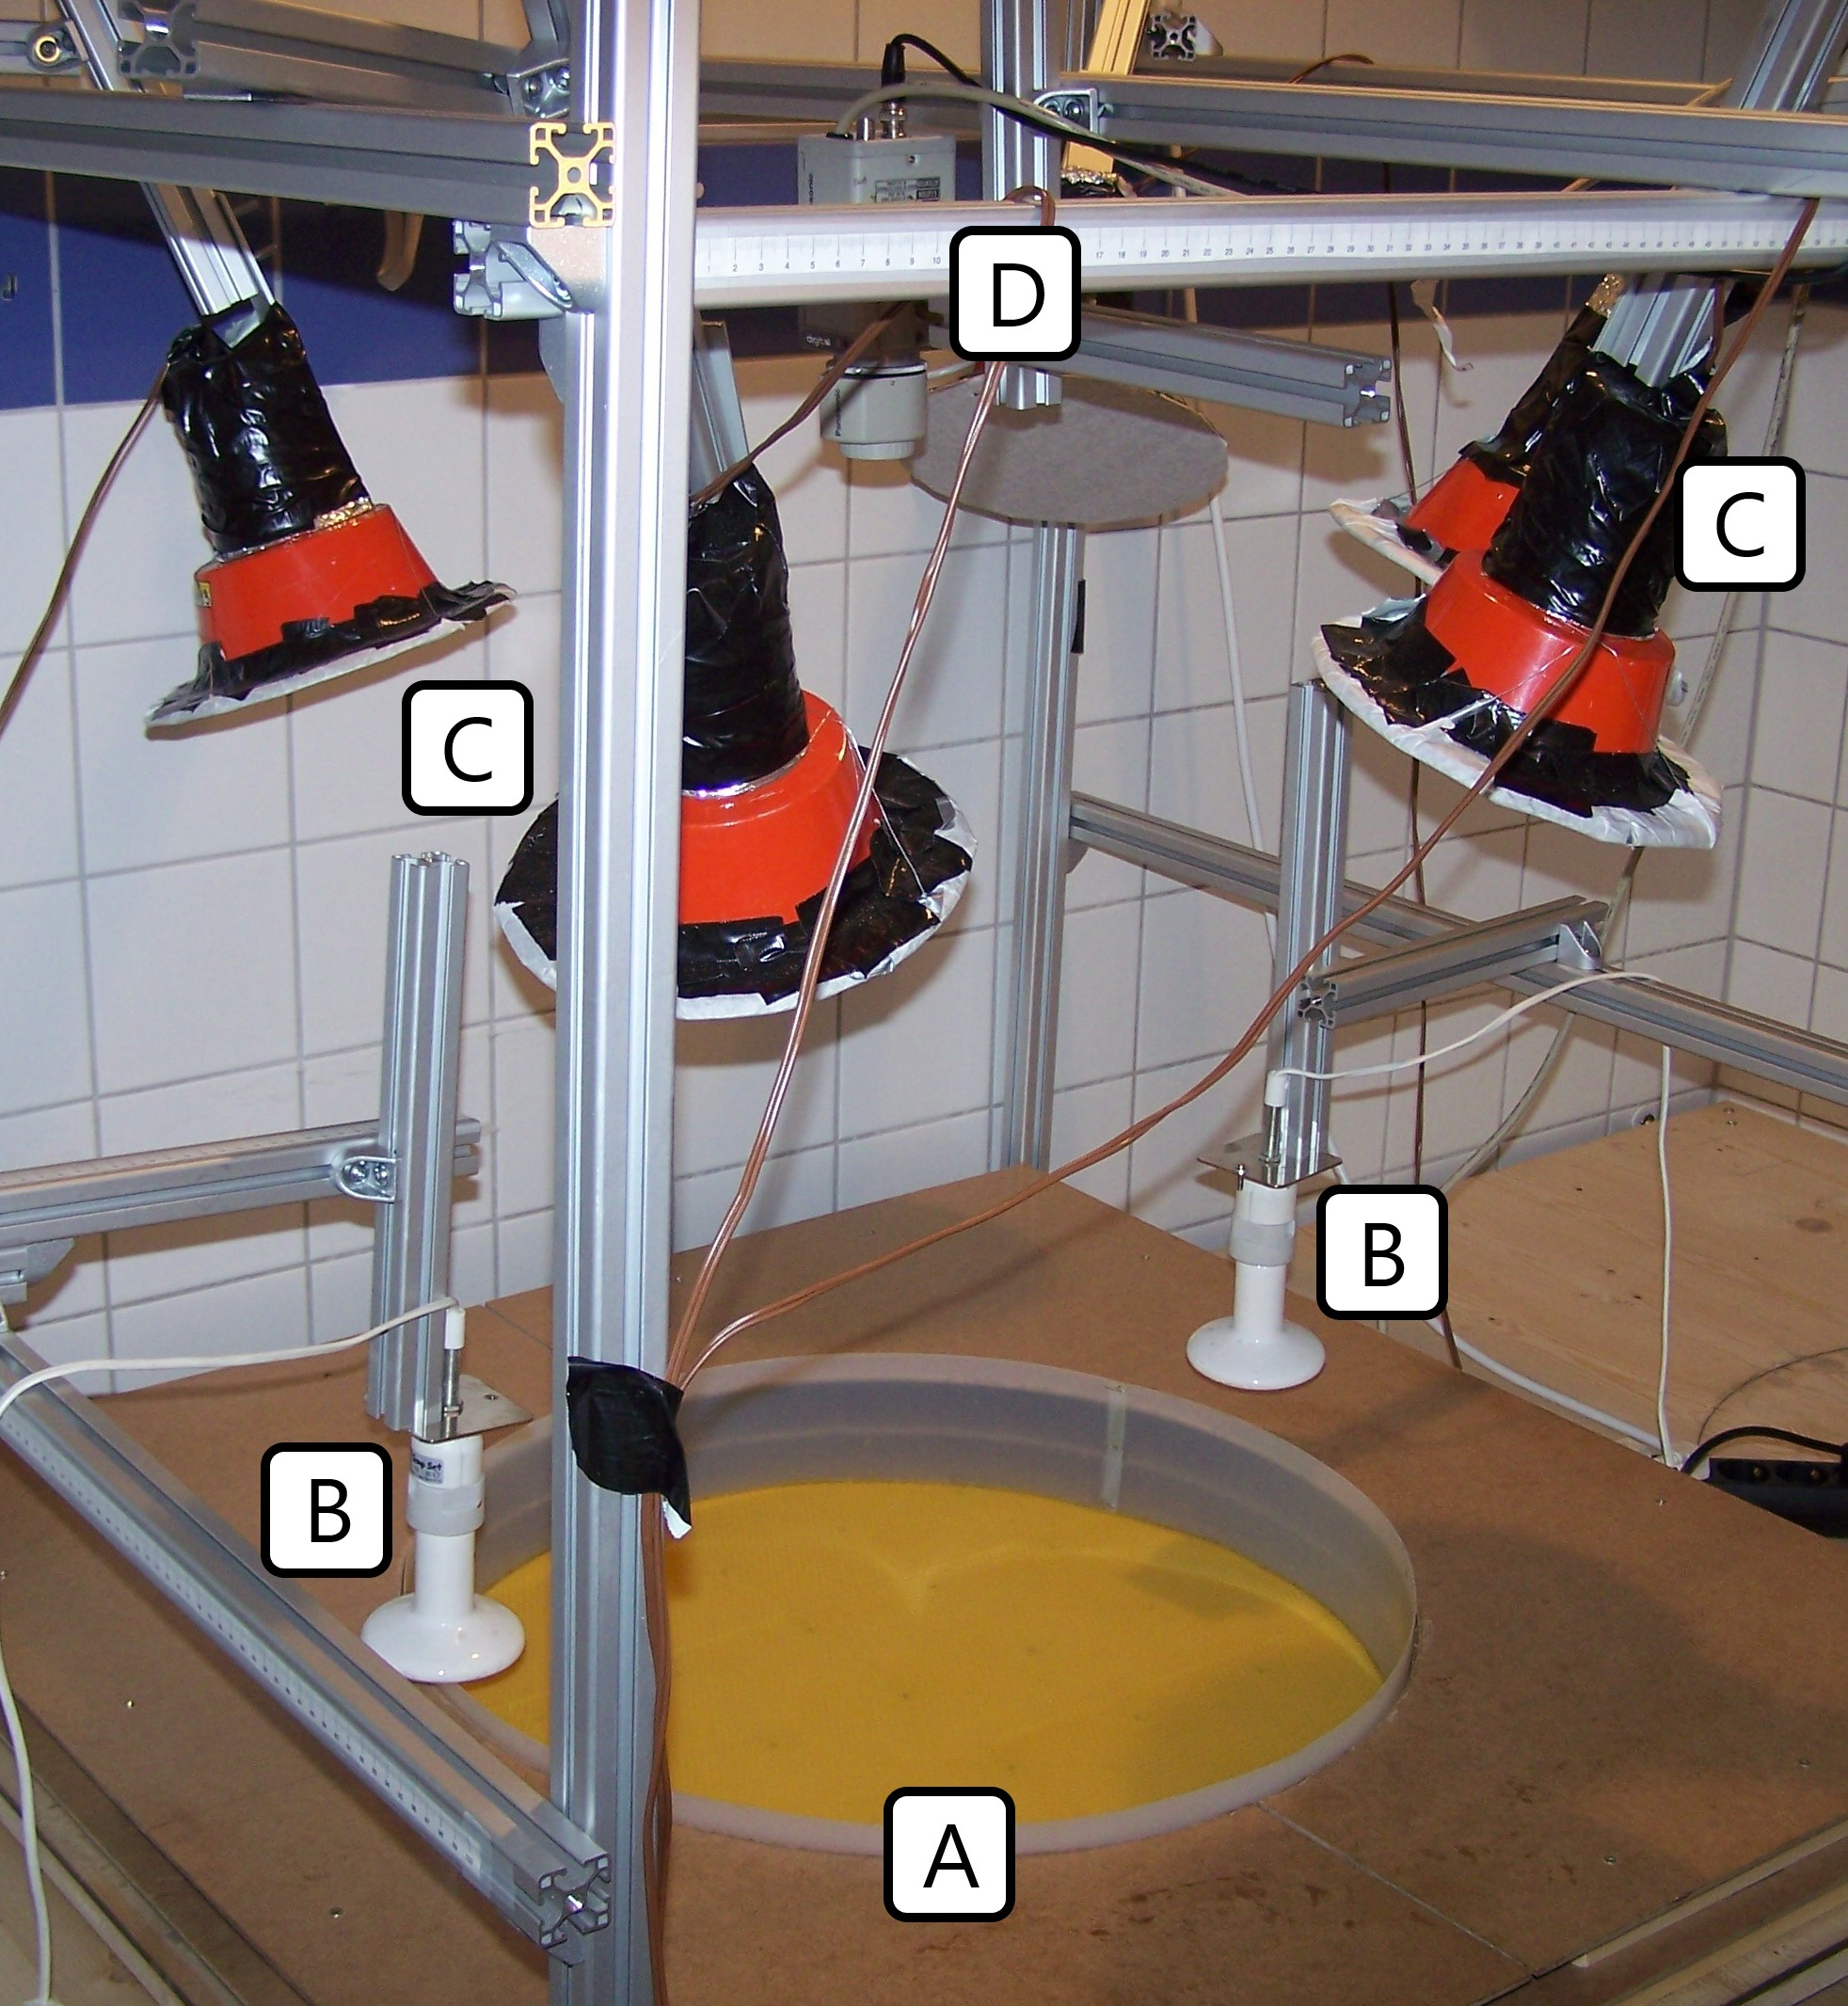
\includegraphics[width=8.7cm, height=10cm]{figures/Setup.jpg}}
    \caption{Setup with: [A] the arena itself with a circular boundary and the temperature sensors ordered in a grid with grid distance d=10cm; [B] the heating elements one on the left above the optimum, and another one on the right above the sub-optimum; [C] lamps that produce diffused red light with a wavelength $\lambda_{0} \approx 700nm$; and [D] a FLIR infrared camera that captures the bees trajectories}
    \label{fig:Setup}
\end{figure}

\section{Experimental Runs}

Although it is known that young honeybees in laboratory experiments prefer a certain ambient temperature \cite{heran1952}, which they usually actively seek, the individual runs only rarely showed a direct uphill walk in the gradient with a subsequent resting phase at the optimal temperature of 36 \textdegree C, which was expected to be the predominant behaviour.
On the contrary it appears that they display a variety of motion trajectories, that at a first glance could be classified into four distinct behavioural types.

The four dominant types of movement, that are present in all individual bees, define the success in finding the optimal spot within the arena. These characteristic movements are often present several times in each experimental run and can be described as following:

\begin{itemize}
    \item Goal Following behaviour (\textbf{GF}): the bee moves towards the optimum with a constant velocity
    \item Immobile behaviour (\textbf{IB}): the bee has a low velocity or none at all
    \item Wall Following behaviour (\textbf{WF}): the bee moves along the boundary with a Gaussian distributed velocity
    \item Random Walking behaviour (\textbf{RW}): the bee moves randomly and with random velocities uphill and downhill through all zones 
\end{itemize}

The 16 given example trajectories in figure \ref{fig:Well_Beehaved} are instances where subjectively one of the behaviours was more prevalent than the others, four for each of the four types.
\\
However, it is necessary to mention here already, that most of the bees show a combination of those different movements, often randomly changing between them, which mostly eradicates the attempt to classify a bee purely as an uphill or random walker. Nevertheless, the collocation of the movement types and their order definitely affect the success of a bee to actually spend most of its experimental run-time within a satisfactory ambient temperature and heterogeneous swarms, where individual behaviours differ from one to another, are suspected to outperform their homogeneous counterparts. \cite{Kengyel2015} 
\begin{figure}
    \centering
    \frame{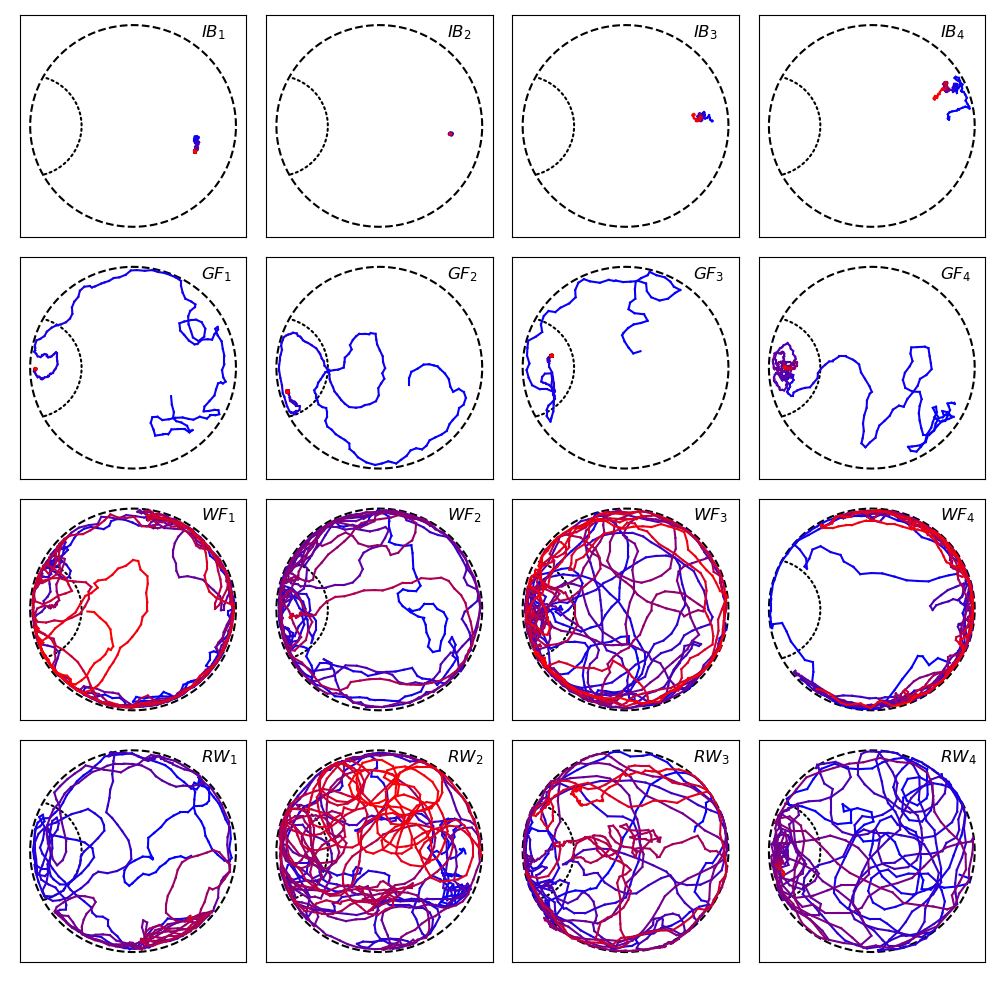
\includegraphics[width=14.7cm, height=14.7cm]{figures/Well_Beehaved.png}}
    \caption{Shown are 16 different trajectories, subjectively categorized into four different behavioural types by trained human perception. For each type (IB or immobile, GF or goal following, WF or wall following and RW or random walking behaviour) we chose four representative trajectories. Each trajectory is color coded over the whole run of the experiment, with blue being the color at the beginning of the run, gradually reaching red at the end of it. The dashed line represents the wall of the arena and the dotted line represents the warmest area (or temperature optimum) within it.}
    \label{fig:Well_Beehaved}
\end{figure}



